%Design Options
\section{ADCS}
\label{sect_adcs}
The design of the \ac{ADCS} is twofold. On one side there is the attitude determination, on the other the attitude control. With the attitude determination the state (attitude and attitude rate) of the satellite is established, if the state of the satellite is not as it should be the attitude control part adapts the attitude. It is also possible to have a passive system by using the gravity gradient of the Earth, using the Earth's magnetic field or by having a spinning spacecraft. In all cases the satellite is only stable along two axis. A design option tree can be found in figure \ref{pic_DOTadcs} on page \pageref{pic_DOTadcs}.

\subsection{Attitude determination}
For attitude determination a number of different sensors could be used. First of all there are inertial measurement units like gyroscopes and accelerometers. These systems measure the attitude deviation from a set point in time. Then there are Sun sensors, which use the position and angle towards the Sun,  Earth scanners scan the Earth's limb, Star trackers use the positions of known stars to determine the attitude of the satellite. A recent technique to determine the attitude is using accurate relative \ac{GPS} measurements with multiple antennas on the satellite body.

\subsection{Attitude control}
The attitude control is able to change the attitude of the satellite. Basically there are four kinds of active systems to do this: using thrusters, momentum wheels magnetic torques and \acp{CMG}. Thrusters exert gasses and momentum wheels spin up to to give a momentum to the satellite. In magnetic torquers a current through a coil produces a Lorentz force, using the magnetic field of the Earth. Because there is no friction, an equal amount of momentum has to be added in the other direction as well to stabilise the attitude again. \ac{CMG}s have a constant speed, but the angle in which the force vector is directed is adapted by a single or double set of gimbals. Passive means of attitude control include gravity gradient, spin stabilisation and passive magnetic. Due to the Earth's gravity field gravity gradient satellites will always tend to point towards Earth with their smallest moment of inertia axis. Spin stabilised spacecraft are rotating around one axis to stabilise along the other two. Passive magnetic stabilising uses the magnetic field of the Earth and permanent magnets for its stabilisation. Passive means of stabilisation are often only usable for stabilisation along two axis, if stabilisation or even control along three axis is required a different system is required.

\begin{figure}
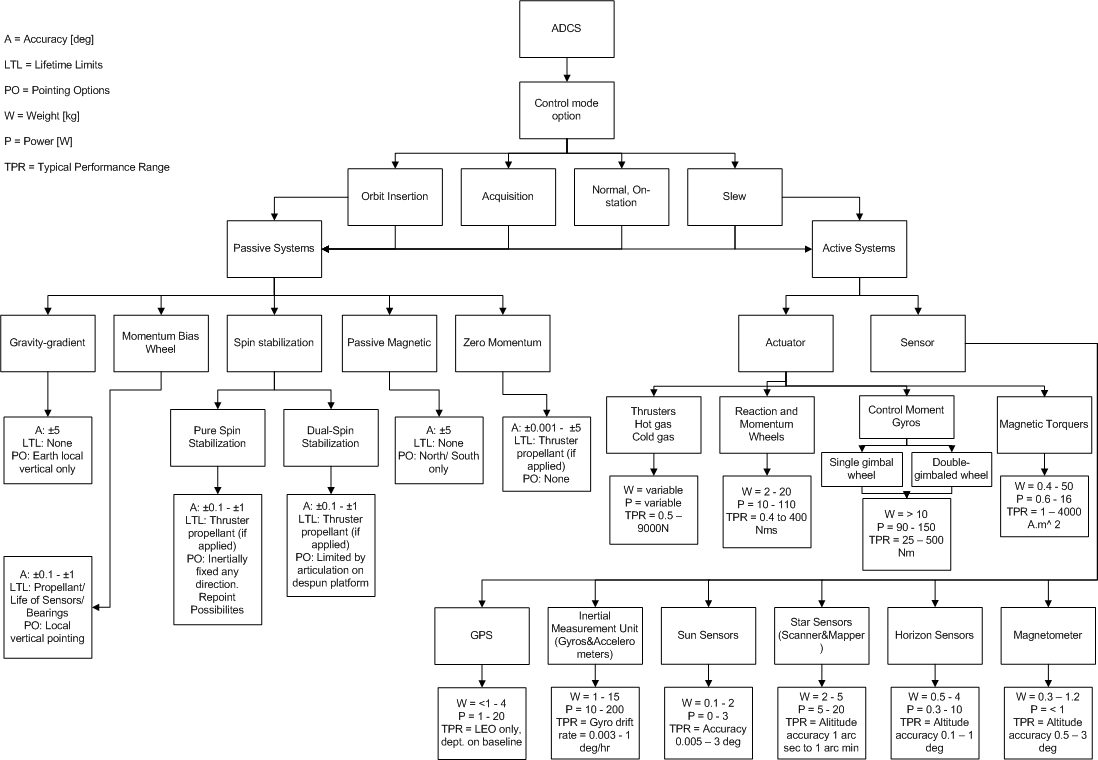
\includegraphics[width=0.8\textwidth, angle=90]{img/DOTadcs.png}
\caption{Design option tree for the \ac{ADCS}}
\label{pic_DOTadcs}
\end{figure}